\begin{appendices}




\section{Παράρτημα - Node Modules}


\label{appendix:Node_modules}
\begin{table}[H]
\centering
    \begin{tabularx}{\textwidth}{ | c | X | } 

    \hline
    Symbol & Function\\
    \hline
    
    % ----------------------------------------------------
    \_gpx &
    \begin{tabular}{@{}c@{}}
        $g_i = a_i * b_i$\\
        $p_i = a_i + b_i$\\
        $x_i = a_i \oplus b_i $
    \end{tabular}\\\hline
    
    % ----------------------------------------------------
    \_4g2p\_R4 &
    \begin{tabular}{@{}c@{}}
        $R = g_3 + g_2 + p_1g_1 + p_1p_0g_0$
    \end{tabular}\\\hline
    
    % ----------------------------------------------------
    \_4p\_Q4 &
    \begin{tabular}{@{}c@{}}
        $Q = p_3 p_2 p_1 p_0$
    \end{tabular}\\\hline
    
    % ----------------------------------------------------
    \_4R2Q\_R4 &
    \begin{tabular}{@{}c@{}}
        $R = R_3 + R_2 + Q_1R_1 + Q_1Q_0R_0$
    \end{tabular}\\\hline
    
    % ----------------------------------------------------
    \_D16 &
    \begin{tabular}{@{}c@{}}
        $D = p_1R + p_0Q$
    \end{tabular}\\\hline
    
    % ----------------------------------------------------
    \_Jsum &
    \begin{tabular}{@{}c@{}}
        $sum = R\ ?\ x\oplus D\ :\ x$
    \end{tabular}\\\hline
    
    % ----------------------------------------------------
    \_1R4Q\_Q4 &
    \begin{tabular}{@{}c@{}}
        $Q = Q_3 Q_2 Q_1 (Q_0 + R)$
    \end{tabular}\\\hline
    
    % ----------------------------------------------------
    \_D64\_1 &
    \begin{tabular}{@{}c@{}}
        $D = g_1 + p_2g_0 + p_2p_1p_0$
    \end{tabular}\\\hline
    
    % ----------------------------------------------------
    \_D64\_2 &
    \begin{tabular}{@{}c@{}}
        $D = D (R + Q)$
    \end{tabular}\\\hline
    
    % ----------------------------------------------------
    \_2g\_R2 &
    \begin{tabular}{@{}c@{}}
        $R = g_1 + g_0$
    \end{tabular}\\\hline
    
    % ----------------------------------------------------
    \_2p\_Q2 &
    \begin{tabular}{@{}c@{}}
        $Q = p_1p_0$
    \end{tabular}\\\hline
    
    % ----------------------------------------------------
    \_4g2p\_H4 &
    \begin{tabular}{@{}c@{}}
        $H = g_3 + g_2 + p_1g_1 + p_1p_0g_0$
    \end{tabular}\\\hline
    
    % ----------------------------------------------------
    \_P4 &
    \begin{tabular}{@{}c@{}}
        $P = p_3p_2p_1p_0$
    \end{tabular}\\\hline
    
    % ----------------------------------------------------
    \_4G3P\_G4 &
    \begin{tabular}{@{}c@{}}
        $G = G_3 + P_2G_2 + P_2P_1G_1 + P_2P_1P_0G_0$
    \end{tabular}\\\hline
    
    % ----------------------------------------------------
    \_Lsum &
    \begin{tabular}{@{}c@{}}
        $sum = H\ ?\ x \oplus p\ :\ x$
    \end{tabular}\\\hline
    
    % ----------------------------------------------------
    \_2g\_H2 &
    \begin{tabular}{@{}c@{}}
        $H = g_1 + g_0$
    \end{tabular}\\\hline
    
    % ----------------------------------------------------
    \_2p\_P2 &
    \begin{tabular}{@{}c@{}}
        $P = p_1 p_0$
    \end{tabular}\\\hline
    
    % ----------------------------------------------------
    \_Psum &
    \begin{tabular}{@{}c@{}}
        $sum = G \oplus x$
    \end{tabular}\\\hline
    
    % ----------------------------------------------------
    \_2g1p\_G2 &
    \begin{tabular}{@{}c@{}}
        $G = g_1 + p*g_0$
    \end{tabular}\\\hline
    
    % ----------------------------------------------------
    \_2R1Q\_R2 &
    \begin{tabular}{@{}c@{}}
        $R = R_1 + Q*R_0$
    \end{tabular}\\\hline
    
    
    \end{tabularx}
    \caption{Modules Description}
    \label{table:node_modules}
\end{table}

\end{appendices}
% \subsection{Schematics}

% \thispagestyle{empty}

% \begin{figure}[H]
%     \centering
%     %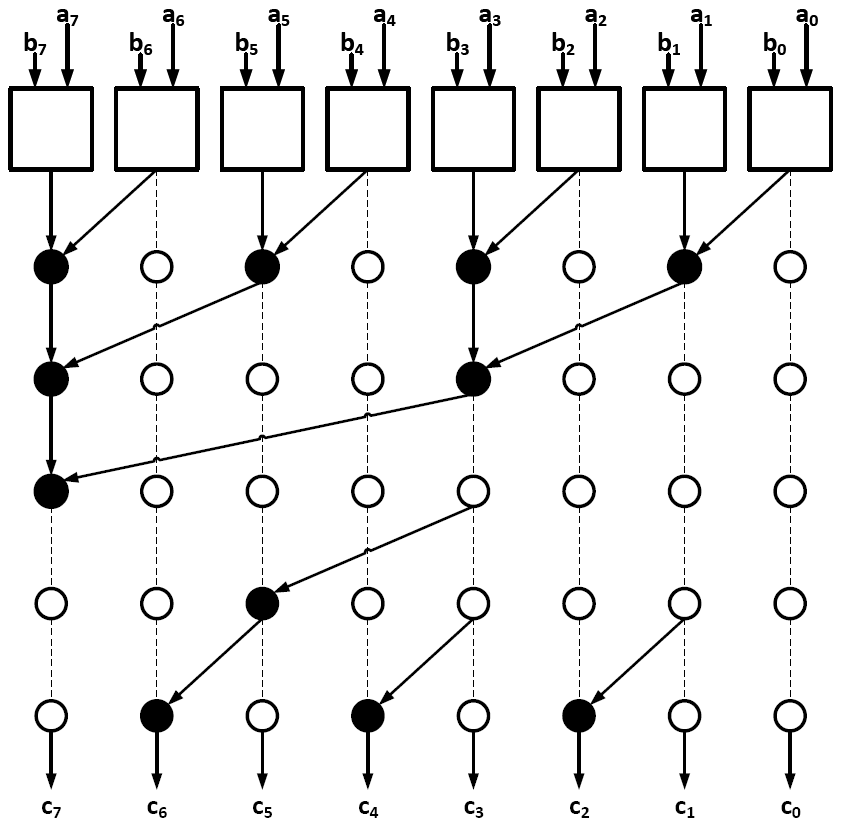
\includegraphics[width=\textwidth]{Brent_Kung_Prefix.png}
%     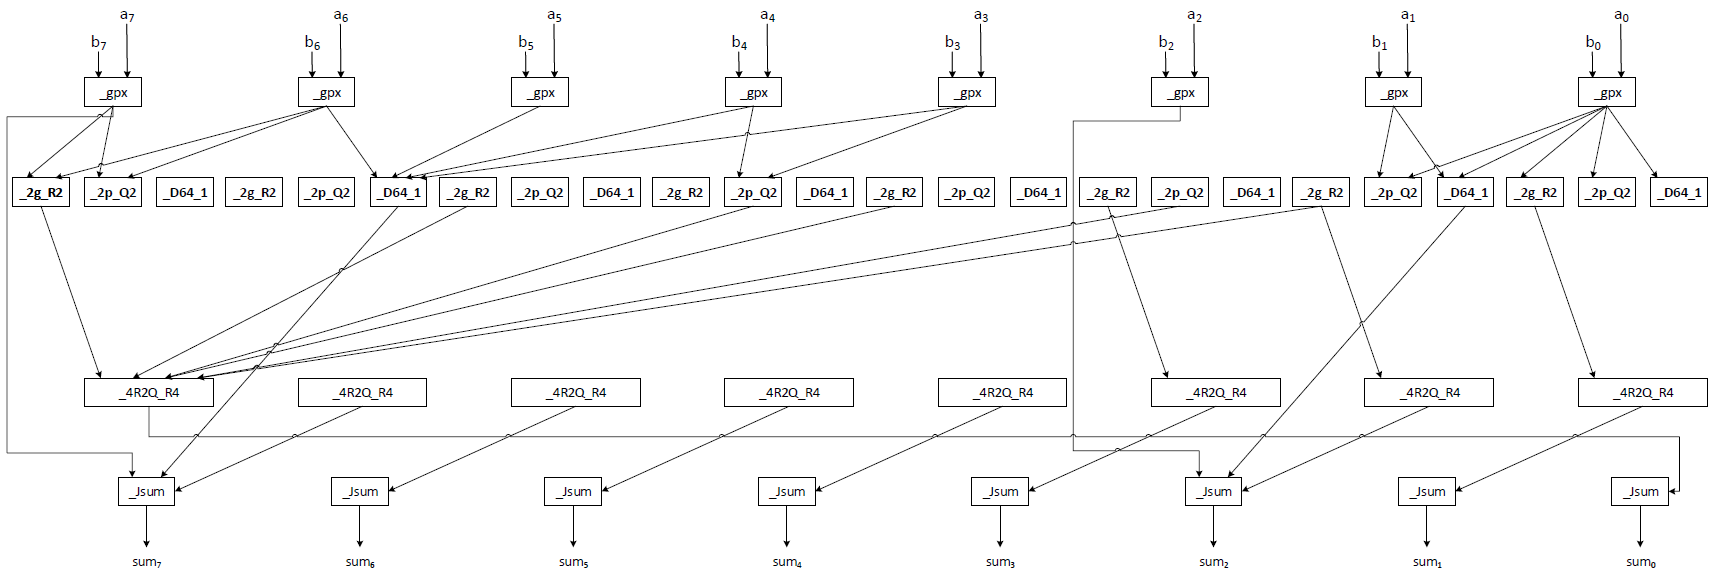
\includegraphics[angle=90,scale=0.5]{Pictures/J8_Adder.png}
%     \caption{Jackson 8-bit $2^n-1$ Adder}
%     \label{Schematic:Jackson_8}
% \end{figure}